% Options for packages loaded elsewhere
\PassOptionsToPackage{unicode}{hyperref}
\PassOptionsToPackage{hyphens}{url}
\PassOptionsToPackage{dvipsnames,svgnames,x11names}{xcolor}
%
\documentclass[
]{agujournal2019}

\usepackage{amsmath,amssymb}
\usepackage{iftex}
\ifPDFTeX
  \usepackage[T1]{fontenc}
  \usepackage[utf8]{inputenc}
  \usepackage{textcomp} % provide euro and other symbols
\else % if luatex or xetex
  \usepackage{unicode-math}
  \defaultfontfeatures{Scale=MatchLowercase}
  \defaultfontfeatures[\rmfamily]{Ligatures=TeX,Scale=1}
\fi
\usepackage{lmodern}
\ifPDFTeX\else  
    % xetex/luatex font selection
\fi
% Use upquote if available, for straight quotes in verbatim environments
\IfFileExists{upquote.sty}{\usepackage{upquote}}{}
\IfFileExists{microtype.sty}{% use microtype if available
  \usepackage[]{microtype}
  \UseMicrotypeSet[protrusion]{basicmath} % disable protrusion for tt fonts
}{}
\makeatletter
\@ifundefined{KOMAClassName}{% if non-KOMA class
  \IfFileExists{parskip.sty}{%
    \usepackage{parskip}
  }{% else
    \setlength{\parindent}{0pt}
    \setlength{\parskip}{6pt plus 2pt minus 1pt}}
}{% if KOMA class
  \KOMAoptions{parskip=half}}
\makeatother
\usepackage{xcolor}
\setlength{\emergencystretch}{3em} % prevent overfull lines
\setcounter{secnumdepth}{5}
% Make \paragraph and \subparagraph free-standing
\ifx\paragraph\undefined\else
  \let\oldparagraph\paragraph
  \renewcommand{\paragraph}[1]{\oldparagraph{#1}\mbox{}}
\fi
\ifx\subparagraph\undefined\else
  \let\oldsubparagraph\subparagraph
  \renewcommand{\subparagraph}[1]{\oldsubparagraph{#1}\mbox{}}
\fi


\providecommand{\tightlist}{%
  \setlength{\itemsep}{0pt}\setlength{\parskip}{0pt}}\usepackage{longtable,booktabs,array}
\usepackage{calc} % for calculating minipage widths
% Correct order of tables after \paragraph or \subparagraph
\usepackage{etoolbox}
\makeatletter
\patchcmd\longtable{\par}{\if@noskipsec\mbox{}\fi\par}{}{}
\makeatother
% Allow footnotes in longtable head/foot
\IfFileExists{footnotehyper.sty}{\usepackage{footnotehyper}}{\usepackage{footnote}}
\makesavenoteenv{longtable}
\usepackage{graphicx}
\makeatletter
\def\maxwidth{\ifdim\Gin@nat@width>\linewidth\linewidth\else\Gin@nat@width\fi}
\def\maxheight{\ifdim\Gin@nat@height>\textheight\textheight\else\Gin@nat@height\fi}
\makeatother
% Scale images if necessary, so that they will not overflow the page
% margins by default, and it is still possible to overwrite the defaults
% using explicit options in \includegraphics[width, height, ...]{}
\setkeys{Gin}{width=\maxwidth,height=\maxheight,keepaspectratio}
% Set default figure placement to htbp
\makeatletter
\def\fps@figure{htbp}
\makeatother
% definitions for citeproc citations
\NewDocumentCommand\citeproctext{}{}
\NewDocumentCommand\citeproc{mm}{%
  \begingroup\def\citeproctext{#2}\cite{#1}\endgroup}
\makeatletter
 % allow citations to break across lines
 \let\@cite@ofmt\@firstofone
 % avoid brackets around text for \cite:
 \def\@biblabel#1{}
 \def\@cite#1#2{{#1\if@tempswa , #2\fi}}
\makeatother
\newlength{\cslhangindent}
\setlength{\cslhangindent}{1.5em}
\newlength{\csllabelwidth}
\setlength{\csllabelwidth}{3em}
\newenvironment{CSLReferences}[2] % #1 hanging-indent, #2 entry-spacing
 {\begin{list}{}{%
  \setlength{\itemindent}{0pt}
  \setlength{\leftmargin}{0pt}
  \setlength{\parsep}{0pt}
  % turn on hanging indent if param 1 is 1
  \ifodd #1
   \setlength{\leftmargin}{\cslhangindent}
   \setlength{\itemindent}{-1\cslhangindent}
  \fi
  % set entry spacing
  \setlength{\itemsep}{#2\baselineskip}}}
 {\end{list}}
\usepackage{calc}
\newcommand{\CSLBlock}[1]{\hfill\break\parbox[t]{\linewidth}{\strut\ignorespaces#1\strut}}
\newcommand{\CSLLeftMargin}[1]{\parbox[t]{\csllabelwidth}{\strut#1\strut}}
\newcommand{\CSLRightInline}[1]{\parbox[t]{\linewidth - \csllabelwidth}{\strut#1\strut}}
\newcommand{\CSLIndent}[1]{\hspace{\cslhangindent}#1}

\usepackage{url} %this package should fix any errors with URLs in refs.
\usepackage{lineno}
\usepackage[inline]{trackchanges} %for better track changes. finalnew option will compile document with changes incorporated.
\usepackage{soul}
\linenumbers
\makeatletter
\@ifpackageloaded{caption}{}{\usepackage{caption}}
\AtBeginDocument{%
\ifdefined\contentsname
  \renewcommand*\contentsname{Table of contents}
\else
  \newcommand\contentsname{Table of contents}
\fi
\ifdefined\listfigurename
  \renewcommand*\listfigurename{List of Figures}
\else
  \newcommand\listfigurename{List of Figures}
\fi
\ifdefined\listtablename
  \renewcommand*\listtablename{List of Tables}
\else
  \newcommand\listtablename{List of Tables}
\fi
\ifdefined\figurename
  \renewcommand*\figurename{Figure}
\else
  \newcommand\figurename{Figure}
\fi
\ifdefined\tablename
  \renewcommand*\tablename{Table}
\else
  \newcommand\tablename{Table}
\fi
}
\@ifpackageloaded{float}{}{\usepackage{float}}
\floatstyle{ruled}
\@ifundefined{c@chapter}{\newfloat{codelisting}{h}{lop}}{\newfloat{codelisting}{h}{lop}[chapter]}
\floatname{codelisting}{Listing}
\newcommand*\listoflistings{\listof{codelisting}{List of Listings}}
\makeatother
\makeatletter
\makeatother
\makeatletter
\@ifpackageloaded{caption}{}{\usepackage{caption}}
\@ifpackageloaded{subcaption}{}{\usepackage{subcaption}}
\makeatother
\ifLuaTeX
  \usepackage{selnolig}  % disable illegal ligatures
\fi
\usepackage{bookmark}

\IfFileExists{xurl.sty}{\usepackage{xurl}}{} % add URL line breaks if available
\urlstyle{same} % disable monospaced font for URLs
\hypersetup{
  pdftitle={Temporal and spatial variations of PM2 and PM10 concentrations in Mongolia},
  pdfauthor={Erdenebayar Munkhtsetseg; Atsushi Shimizu},
  pdfkeywords={particulate matters, concentrations of PM10 and PM2.5},
  colorlinks=true,
  linkcolor={blue},
  filecolor={Maroon},
  citecolor={Blue},
  urlcolor={Blue},
  pdfcreator={LaTeX via pandoc}}

\journalname{Earth and Space Science}

\draftfalse

\begin{document}
\title{Temporal and spatial variations of PM2 and PM10 concentrations in
Mongolia}

\authors{Erdenebayar Munkhtsetseg\affil{1,2}, Atsushi Shimizu\affil{3}}
\affiliation{1}{National University of Mongolia (NUM),
Mongolia, }\affiliation{2}{Kanazawa University,
Japan, }\affiliation{3}{National Institute for Environmental Studies
(NIES), Japan, }
\correspondingauthor{Atsushi Shimizu}{shimizua@nies.go.jp}


\begin{abstract}
PM2.5 and PM10 data for the 4 distinct sites of Mongolia from 2008 to
2020 is found \ldots. \ldots{}
\end{abstract}

\section*{Plain Language Summary}
PM2.5 and PM10 data for the 4 distinct sites of Mongolia from 2008 to
2020 is found \ldots{}



\subsection{Data \& Methods}\label{sec-data-methods}

\section{01\_datawork}\label{datawork}

Munkhtsetseg

Library

\section{Import the dataset and remove the
duplicates}\label{import-the-dataset-and-remove-the-duplicates}

Import the dataset from the directory of: \textasciitilde/Data
Input/Preprocessing data/Preprocessing data.csv, assign the dataset as
object of df:

Remove the duplicates with the function of distinct(), assign the
dataset as df\_01:

\subsection{Produce a table with missing
data}\label{produce-a-table-with-missing-data}

For date options as year, month, etc:

\begin{verbatim}
# A tibble: 35 × 9
# Groups:   Station.name [4]
   Station.name  Year NA_date NA_PM2 NA_PM10 NA_Vis NA_WD NA_WS NA_OPC
   <chr>        <int>   <int>  <int>   <int>  <int> <int> <int>  <int>
 1 Dalanzadgad   2009    8760    715     929    659   748   748   8760
 2 Dalanzadgad   2010    8784    921    1086    756   787   787   8784
 3 Dalanzadgad   2011    8760   2652    3309   1759  2394  2394   8760
 4 Dalanzadgad   2012    5088   1074    3016    693  1412  1412   5088
 5 Dalanzadgad   2013    6096   1766    1809   2479  1240  1240   6096
 6 Dalanzadgad   2014    7800    843     921   6068  1482  1482   7800
 7 Dalanzadgad   2015    8760   1539    1587   8115  2635  2635   8760
 8 Dalanzadgad   2016    6288   1654    1613   5995  3306  3306   6288
 9 Sainshand     2009    8688    376     424    423   587   587   8688
10 Sainshand     2010    8784   2557    2577   1113  1210  1210   8784
# ℹ 25 more rows
\end{verbatim}

For station

\begin{verbatim}
# A tibble: 4 × 8
  Station.name NA_date NA_PM2 NA_PM10 NA_Vis NA_WD NA_WS NA_OPC
  <chr>          <int>  <int>   <int>  <int> <int> <int>  <int>
1 Dalanzadgad    60336  11164   14270  26524 14004 14004  60336
2 Sainshand      59040  11727   11929   9320  8527  8527  59040
3 UB             76656   7879    8716   3770  4053  4053  43415
4 Zamynuud       67392   8880   10075   3444  4960  4960  67392
\end{verbatim}

By percentages

\begin{verbatim}
# A tibble: 4 × 6
# Groups:   Station.name [4]
  Station.name missing_PM2 missing_PM10 missing_Vis missing_WS missing_WD
  <chr>              <dbl>        <dbl>       <dbl>      <dbl>      <dbl>
1 Dalanzadgad         25.7         19.2       44.5       24.3       24.3 
2 Sainshand           20.0         19.7       15.7       14.6       14.6 
3 UB                  11.9         11.0        4.53       4.85       4.85
4 Zamynuud            14.4         12.7        5.49       7.44       7.44
\end{verbatim}

\section{Note that:}\label{note-that}

We use the data in the period of 2009-2018, which has been regarded as a
monitoring work stabilized since 2008 when is the beginning of the
monitoring. According to NIES, site maintenance was consistent up to
2018. - Sainshand site, data 2009-2015 get used; - Dalanzad site:
2009-2016. - UB: 2009-2018 - Zamyn uud: 2009-2018

\section{Remove the spikes, and produce an extended
table}\label{remove-the-spikes-and-produce-an-extended-table}

Remove the spikes in the datasets, and produce the table with NA, with
removed spikes; express it in a percentages. \#\#\# Remove the spikes
Method 1. Mean value +- (3-5)SD - Find Monthly mean

\begin{verbatim}
# A tibble: 1,798 × 12
    Year Month   Day  Hour PM2   PM10  Visibility    WD    WS   OPC Station.name
   <int> <int> <int> <int> <chr> <chr>      <int> <int> <dbl> <int> <chr>       
 1  2009     1     2    17 Outl… 0.29        3622   141 0.524    NA UB          
 2  2009     1     3    12 Outl… 0.446       2399   109 0.117    NA UB          
 3  2009     1     3    13 Outl… 0.288       1347    17 0.492    NA UB          
 4  2009     1     3    14 Outl… 0.504       1241    12 0.829    NA UB          
 5  2009     1     3    15 Outl… 0.478       1341    11 0.39     NA UB          
 6  2009     1     3    16 Outl… 0.449       2945   136 0.123    NA UB          
 7  2009     1     3    18 Outl… 0.341       1436    13 0.742    NA UB          
 8  2009     1     3    19 Outl… 0.397       1847    13 0.453    NA UB          
 9  2009     1     3    20 Outl… 0.297       3359    22 0.462    NA UB          
10  2009     1     4     2 Outl… 0.311       3167    96 0.759    NA UB          
# ℹ 1,788 more rows
# ℹ 1 more variable: Date <chr>
\end{verbatim}

\begin{verbatim}
# A tibble: 4,014 × 12
    Year Month   Day  Hour PM2   PM10  Visibility    WD    WS   OPC Station.name
   <int> <int> <int> <int> <chr> <chr>      <int> <int> <dbl> <int> <chr>       
 1  2009     1     3    15 Outl… 0.292       3444   119 0.856    NA Dalanzadgad 
 2  2009     1     5    13 Outl… 0.419       1383   260 1.7      NA Dalanzadgad 
 3  2009     1     5    14 Outl… 0.415       1072   266 1.84     NA Dalanzadgad 
 4  2009     1     5    15 Outl… 0.466       1099   261 0.83     NA Dalanzadgad 
 5  2009     1     5    16 Outl… 0.509       1814   260 0.788    NA Dalanzadgad 
 6  2009     1     6     0 Outl… 0.547        744   248 1.23     NA Dalanzadgad 
 7  2009     1     6     1 Outl… 0.728       1093   277 0.738    NA Dalanzadgad 
 8  2009     1     6     2 Outl… 0.597       1723     0 1.62     NA Dalanzadgad 
 9  2009     1     6     3 Outl… 0.33        8186    95 1.1      NA Dalanzadgad 
10  2009     1     6    11 Outl… 0.39        1150   258 1.48     NA Dalanzadgad 
# ℹ 4,004 more rows
# ℹ 1 more variable: Date <chr>
\end{verbatim}

\subsection{Save dataset in folder:
01\_data\_raw}\label{save-dataset-in-folder-01_data_raw}

\section{Tidy data}\label{tidy-data}

\subsection{Fill the missing data}\label{fill-the-missing-data}

Method 1. Fill the gap Method 2. Relationship equation Method 3. Look-up
table

\subsection{Save dataset in folder:
02\_data\_tidy}\label{save-dataset-in-folder-02_data_tidy}

\textsubscript{Source:
\href{https://EmouAcademy.github.io/my-awesome-manuscripts/notebooks/01_datawork-preview.html\#f35a84c0-423e-4e48-bb71-ee0c707df98c}{01\_datawork}}

\subsection{Introduction}\label{introduction}

\textsubscript{Source:
\href{https://EmouAcademy.github.io/my-awesome-manuscripts/index.qmd.html}{Article
Notebook}}

\phantomsection\label{cell-fig-timeline}
\begin{figure}[H]

\centering{

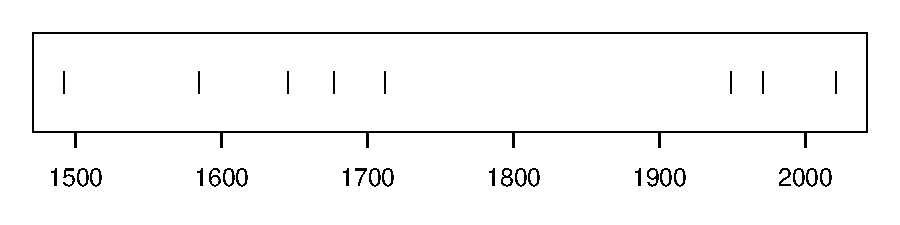
\includegraphics{index_files/figure-pdf/fig-timeline-1.pdf}

}

\caption{\label{fig-timeline}Timeline of recent earthquakes on La Palma}

\end{figure}%

\textsubscript{Source:
\href{https://EmouAcademy.github.io/my-awesome-manuscripts/index.qmd.html}{Article
Notebook}}

\textsubscript{Source:
\href{https://EmouAcademy.github.io/my-awesome-manuscripts/index.qmd.html}{Article
Notebook}}

Based on data up to and including 1971, eruptions on La Palma happen
every 79.8 years on average.

Studies of the magma systems feeding the volcano, such as Marrero et al.
(2019), have proposed that there are two main magma reservoirs feeding
the Cumbre Vieja volcano; one in the mantle (30-40km depth) which
charges and in turn feeds a shallower crustal reservoir (10-20km depth).

Eight eruptions have been recorded since the late 1400s
(Figure~\ref{fig-timeline}).

Data and methods are discussed in Section~\ref{sec-data-methods}.

Let \(x\) denote the number of eruptions in a year. Then, \(x\) can be
modeled by a Poisson distribution

\begin{equation}\phantomsection\label{eq-poisson}{
p(x) = \frac{e^{-\lambda} \lambda^{x}}{x !}
}\end{equation}

where \(\lambda\) is the rate of eruptions per year. Using
Equation~\ref{eq-poisson}, the probability of an eruption in the next
\(t\) years can be calculated.

\begin{longtable}[]{@{}ll@{}}
\caption{Recent historic eruptions on La
Palma}\label{tbl-history}\tabularnewline
\toprule\noalign{}
Name & Year \\
\midrule\noalign{}
\endfirsthead
\toprule\noalign{}
Name & Year \\
\midrule\noalign{}
\endhead
\bottomrule\noalign{}
\endlastfoot
Current & 2021 \\
Teneguía & 1971 \\
Nambroque & 1949 \\
El Charco & 1712 \\
Volcán San Antonio & 1677 \\
Volcán San Martin & 1646 \\
Tajuya near El Paso & 1585 \\
Montaña Quemada & 1492 \\
\end{longtable}

Table~\ref{tbl-history} summarises the eruptions recorded since the
colonization of the islands by Europeans in the late 1400s.

\begin{figure}

\centering{

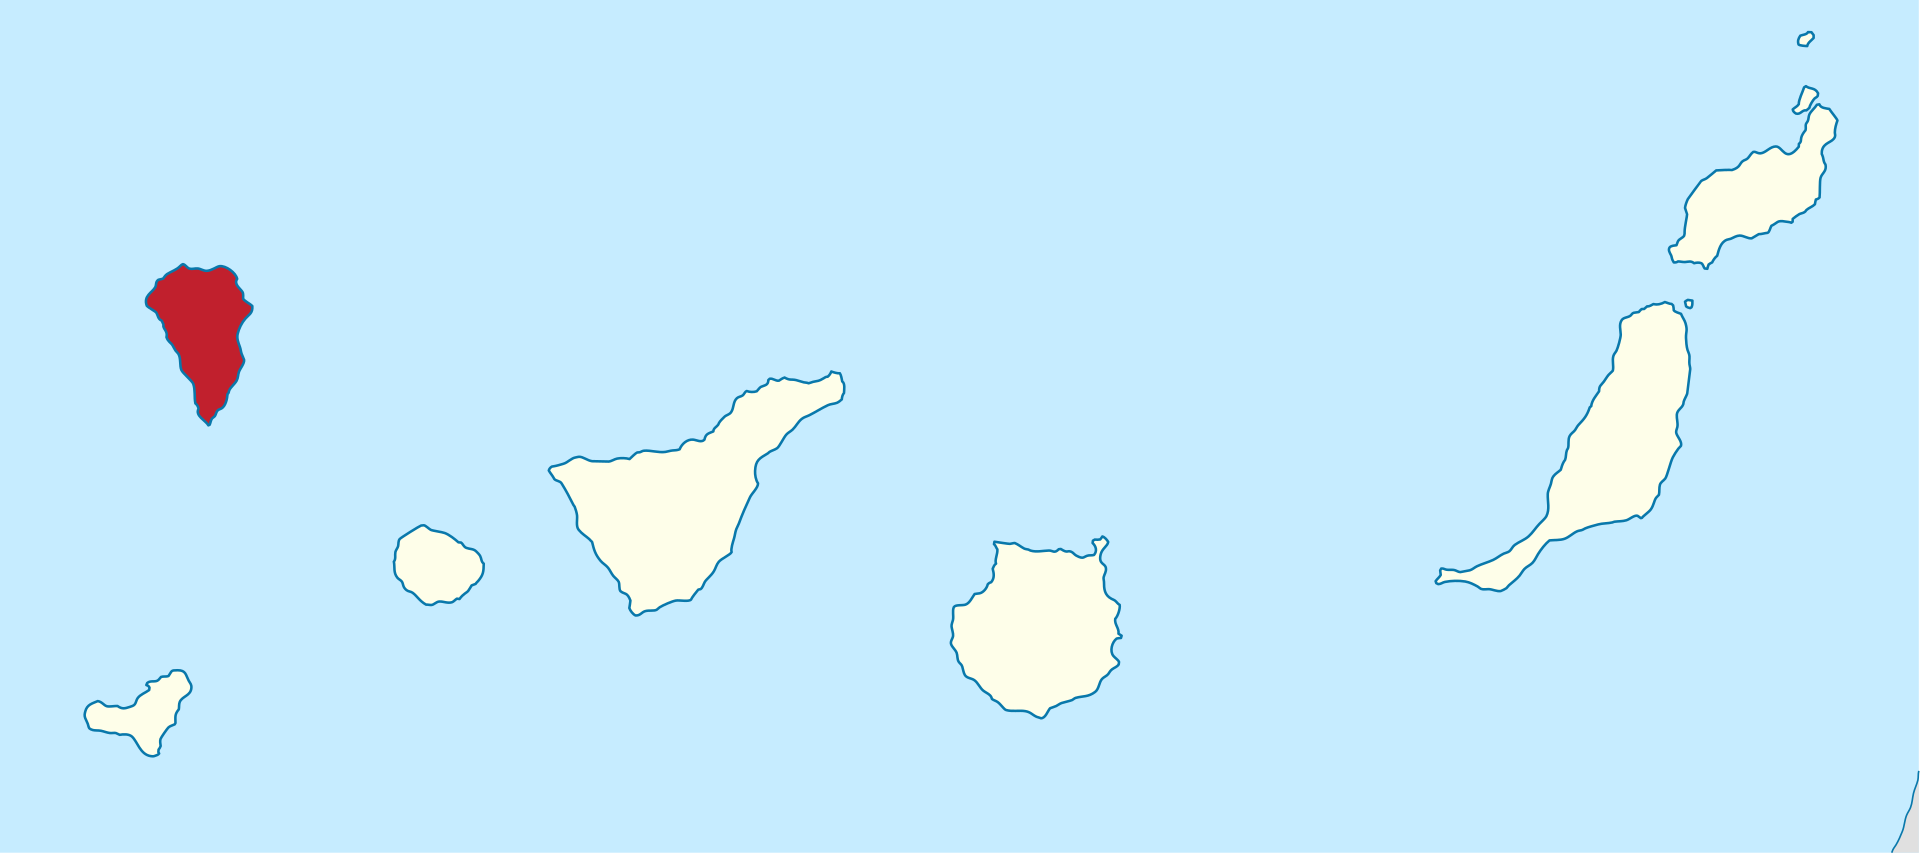
\includegraphics{images/la-palma-map.png}

}

\caption{\label{fig-map}Map of La Palma}

\end{figure}%

La Palma is one of the west most islands in the Volcanic Archipelago of
the Canary Islands (Figure~\ref{fig-map}).

\begin{figure}[H]

\centering{

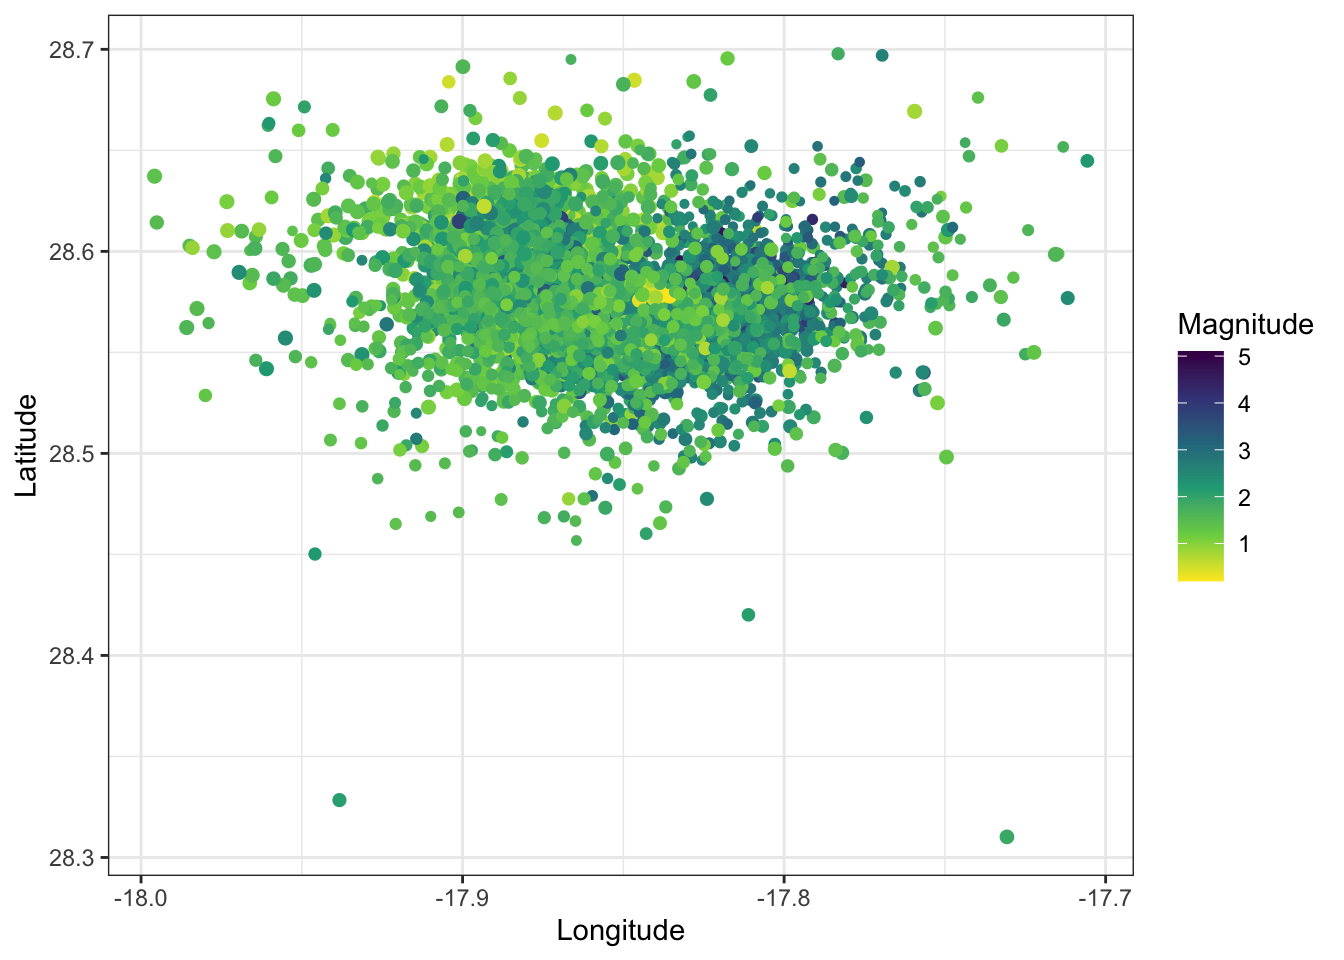
\includegraphics{index_files/figure-latex/notebooks-explore-earthquakes-fig-spatial-plot-output-1.png}

}

\caption{\label{fig-spatial-plot}Locations of earthquakes on La Palma
since 2017}

\end{figure}%

\textsubscript{Source:
\href{https://EmouAcademy.github.io/my-awesome-manuscripts/notebooks/explore-earthquakes-preview.html\#cell-fig-spatial-plot}{Explore
Earthquakes}}

kk

\section{Explore Earthquakes}\label{explore-earthquakes}

Munkhtsetseg

Library

\section{Import the dataset and remove the
duplicates}\label{import-the-dataset-and-remove-the-duplicates-1}

Import the dataset from the directory of: \textasciitilde/Data
Input/Preprocessing data/Preprocessing data.csv, assign the dataset as
object of df:

Remove the duplicates with the function of distinct(), assign the
dataset as df\_01:

\subsection{Produce a table with missing
data}\label{produce-a-table-with-missing-data-1}

For date options as year, month, etc:

\begin{verbatim}
# A tibble: 52 × 9
# Groups:   Station.name [4]
   Station.name  Year NA_date NA_PM2 NA_PM10 NA_Vis NA_WD NA_WS NA_OPC
   <chr>        <int>   <int>  <int>   <int>  <int> <int> <int>  <int>
 1 Dalanzadgad   2008    4630   1543    1672   1463  1566  1566   4630
 2 Dalanzadgad   2009    8760    715     929    659   748   748   8760
 3 Dalanzadgad   2010    8784    921    1086    756   787   787   8784
 4 Dalanzadgad   2011    8760   2652    3309   1759  2394  2394   8760
 5 Dalanzadgad   2012    5088   1074    3016    693  1412  1412   5088
 6 Dalanzadgad   2013    6096   1766    1809   2479  1240  1240   6096
 7 Dalanzadgad   2014    7800    843     921   6068  1482  1482   7800
 8 Dalanzadgad   2015    8760   1539    1587   8115  2635  2635   8760
 9 Dalanzadgad   2016    6288   1654    1613   5995  3306  3306   6288
10 Dalanzadgad   2017    3264     36      45   3264  3264  3264   3264
# ℹ 42 more rows
\end{verbatim}

For station

\begin{verbatim}
# A tibble: 4 × 8
  Station.name NA_date NA_PM2 NA_PM10 NA_Vis NA_WD NA_WS NA_OPC
  <chr>          <int>  <int>   <int>  <int> <int> <int>  <int>
1 Dalanzadgad    69454  13081   16327  32475 20058 20058  69454
2 Sainshand     101230  27588   36117  28986 13768 13768 101230
3 UB             95662   7895    8785   3775  4121  4121  62421
4 Zamynuud       99742  32281   33597  22525  5373  5373  99742
\end{verbatim}

By percentages

\begin{verbatim}
# A tibble: 4 × 2
# Groups:   Station.name [4]
  Station.name   sdq
  <chr>        <dbl>
1 Dalanzadgad   10.7
2 Sainshand     25.9
3 UB            17.9
4 Zamynuud      39.6
\end{verbatim}

Note that the \texttt{echo\ =\ FALSE} parameter was added to the code
chunk to prevent printing of the R code that generated the plot.

\section{Remove the spikes, and produce an extended
table}\label{remove-the-spikes-and-produce-an-extended-table-1}

Remove the spikes in the datasets, and produce the table with NA, with
removed spikes; express it in a percentages.

\subsubsection{Remove the spikes Method 1. Mean value +-
(3-5)SD}\label{remove-the-spikes-method-1.-mean-value---3-5sd}

Method 2. Seasonal variations, and trend-mean

\subsection{Save dataset in folder:
01\_data\_raw}\label{save-dataset-in-folder-01_data_raw-1}

\section{Tidy data}\label{tidy-data-1}

\subsection{Fill the missing data}\label{fill-the-missing-data-1}

Method 1. Fill the gap Method 2. Relationship equation Method 3. Look-up
table

\subsection{Save dataset in folder:
02\_data\_tidy}\label{save-dataset-in-folder-02_data_tidy-1}

Read a clean version of data:

Create spatial plot:

\begin{figure}[H]

\centering{

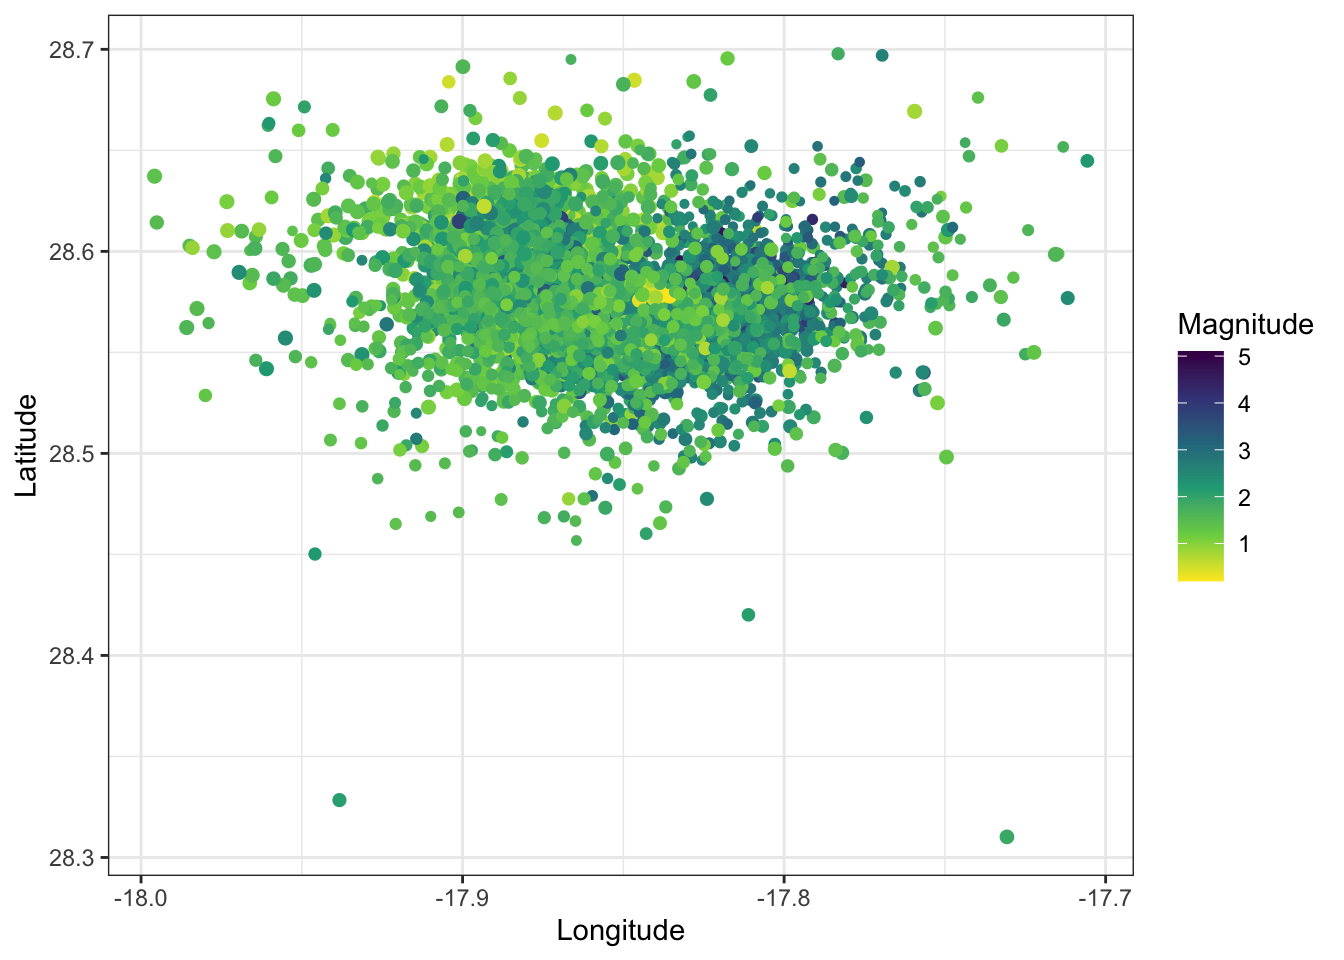
\includegraphics{index_files/figure-latex/notebooks-01-earthquakes-fig-spatial-plot-output-1.png}

}

\caption{\label{fig-spatial-plot}Locations of earthquakes on La Palma
since 2017}

\end{figure}%

\textsubscript{Source:
\href{https://EmouAcademy.github.io/my-awesome-manuscripts/notebooks/01-earthquakes-preview.html\#2671a8ae-4095-42b2-baed-da627795de37}{Explore
Earthquakes}}

Figure~\ref{fig-spatial-plot} shows the location of recent Earthquakes
on La Palma.

\subsection{Results}\label{sec-results}

\subsection{Discussion}\label{sec-discussion}

\subsection{Conclusions}\label{sec-conclusions}

\subsection*{References}\label{references}
\addcontentsline{toc}{subsection}{References}

\phantomsection\label{refs}
\begin{CSLReferences}{1}{0}
\vspace{1em}

\bibitem[\citeproctext]{ref-marrero2019}
Marrero, J., García, A., Berrocoso, M., Llinares, Á., Rodríguez-Losada,
A., \& Ortiz, R. (2019). Strategies for the development of volcanic
hazard maps in monogenetic volcanic fields: The example of {La} {Palma}
({Canary} {Islands}). \emph{Journal of Applied Volcanology}, \emph{8}.
\url{https://doi.org/10.1186/s13617-019-0085-5}

\end{CSLReferences}



\end{document}
